% !TeX encoding = UTF-8
\section{Grundlagen}
\label{sec:Grundlagen}
Dieses Kapitel führt die verwendeten Algorithmen und Berechnungen ein. Anschließend werden die Rahmenbedingungen und die verwendete Hardware und Software vorgestellt.\\
Mit dem A*-Algorithmus wurde schon in den 60er Jahren ein Werkzeug für die Pfadplanung von Robotern eingeführt \citep{astar68}. Pfadplanung bedeutet hier, dass ein Roboter mit festgelegten kinematischen Einschränkungen in einer bestimmten definierten Umgebung von einem Startzustand zu einem Zielzustand mithilfe von Steuerungseingaben gelangen kann, ohne die physikalischen Gesetze zu verletzen oder mit Hindernissen zu kollidieren. Der A*-Algorithmus löst dieses Problem unter gewissen Bedingungen, indem er in einem Graphen den kürzesten Weg zwischen zwei Knoten findet. Allerdings benötigt A* diesen Graphen zur Berechnung des Weges und ist aufgrund des hohen Speicherplatzbedürfnisses für \textit{hochdimensionale Probleme}, d.h. für Probleme mit den oben genannten kinematischen und physikalischen Einschränkungen, nicht geeignet \citep{astar68}.\\
In nachfolgender Zeit wurden \textit{randomisierte Algorithmen} entwickelt, die zwar nicht die mathematisch optimale Lösung lieferten, dafür bedeutende Geschwindigkeitsvorteile hatten. Da in der Praxis oft viele Faktoren, wie z.B. der Luftwiderstand, aufgrund der hohen Komplexität bei geringem Einfluss gar nicht berücksichtigt werden, reicht es, nur bis zu einem gewissen Grade die exakte Lösung zu liefern. \\
Diese Ansätze wurden vom \textit{randomized potential field} Algorithmus \citep{BaLa91} und dem \textit{probalistic roadmap} Algorithmus \citep{AmWu96} verfolgt. Doch auch diese waren nicht allgemein auf \textit{nonholonomic Robots} anwendbar und lösten oft nur spezifische Probleme unter ganz bestimmten Bedingungen. Der Erfolg des \textit{randomized potential field} Algorithmus beispielsweise hing stark von der Wahl einer passenden Heuristik ab \citep[vgl. Kap 3.4 in ][]{BaLa91}. Während sich bei einfachen Ausgangsbedingungen die Heuristik noch einfach finden lies, wurde dies bei komplexen, dynamischen Umgebungen mit Hindernissen und	 physikalischen und kinematischen Bedingungen zu einer großen Herausforderung. \\
1998 schließlich führte Steven LaValle den \textit{RRT}-Algorithmus ein, der die in diesem Kapitel genannten Einschränkungen umgehen sollte.

\subsection{Rapidly-Exploring Random Trees}
\label{RRT}
LaValle erkannte die die Vorteile von randomisierten Algorithmen und die \glqq erfolgreiche Einsetzung im generellen Problem der Pfadplanung\grqq{}. \citep[Kap 1][]{Lav98}. Jedoch sah er auch die Einschränkungen der vorhandenen randomisierten Algorithmen. Insbesondere störte ihn die fehlende Skalierbarkeit in komplexeren und hochdimensionalen Umgebungen, da diese Algorithmen damit nur unter gewissen Vorbedingungen effizient einsetzbar waren. Der \textit{probalistic roadmap} Algorithmus \citep{AmWu96} beispielsweise beinhaltet einen \glqq lokalen Planer\grqq, der zwar für holonomische Systeme und Roboter effiziente Ergebnisse liefert, aber bei nicht holonomischen Fahrzeugen und auf allgemeine Probleme angewendet, schwindet die Effizienz der \textit{probalistic roadmap} \citep{Lav98} .\\
Bei der Entwicklung von \textit{RRT} wurde deshalb viel Wert auf Einfachheit, Allgemeingültigkeit und damit auf Skalierbarkeit gelegt \citep[vlg. Kap 3,][]{Lav98}. Bevor wir jedoch genauer auf die Vorteile des Algorithmus eingehen und warum dieser hier gewählt wurde, folgt jetzt erstmal eine kurze Erklärung der Funktionsweise. 

Der RRT-Algorithmus baut einen Baum auf, indem zufällig gewählte Punkte unter Berücksichtigung einer Metrik verbunden werden. Der Algorithmus mit dem \textit{RRT} $T$, den Eingabeparametern Größe $K$, Metrik $M$, Bewegungsfunktion $u$ und Startzustand \verb|x_init|  funktioniert folgendermaßen:

\subsubsection{Funktionsweise der Rapidly-Exploring Random Trees}
\lstset{language=Pascal, stepnumber=1, numbers=left}
\begin{lstlisting}
BUILD_RRT(K, M, u, x_init)
	T.init (x_init)
	for k=1 to K do
		x_rand = RANDOM_STATE();
		EXTEND(T, x_rand);
	Return T;
\end{lstlisting}
\begin{lstlisting}
EXTEND(T, x)
	x_near = NEAREST_NEIGHBOR(x, T, M);
	x_new = project(x, x_near, u);
	if (Collisionfree(x_new, x_near, u) then
		T.add_vertex(x_new);
		T.add_egde(x_near, x_new, u_new);
		Return Extended;
	else
		Return Trapped;
\end{lstlisting}

Der Baum wird anfangs mit dem Startzustand \verb|x_init| initialisiert, besteht also nur aus dem Knoten \verb|x_init|. Anschließend wird in $K$ Iterationen der Baum $T$ aufgebaut, indem mit \verb|x_rand| ein zufälliger Punkt ausgewählt und mit \verb|EXTEND(T, x_rand)| dem Baum hinzugefügt wird. \\

Die Funktion \verb|EXTEND(T, x)| ermittelt zunächst, wie in Abbildung 1 zu sehen ist, mithilfe der Metrik $M$ den nächsten Nachbar von $x$. Diese Metrik kann von einer einfachen euklidischen Distanz bis hin zur komplexen Einberechnung verschiedener kinematischer Bedingungen alles beinhalten und beeinflusst die Qualität des Baumes sowie die Berechnungsgeschwindigkeit. \\
Vom nächsten Nachbarn \verb|x_near| aus wird mit \verb|project(x,x_near,u)| ein Schritt der Länge  $\epsilon$ in Richtung x durchgeführt und an dieser Stelle der neue Knoten \verb|x_new| erzeugt. 
\begin{figure}
\centering
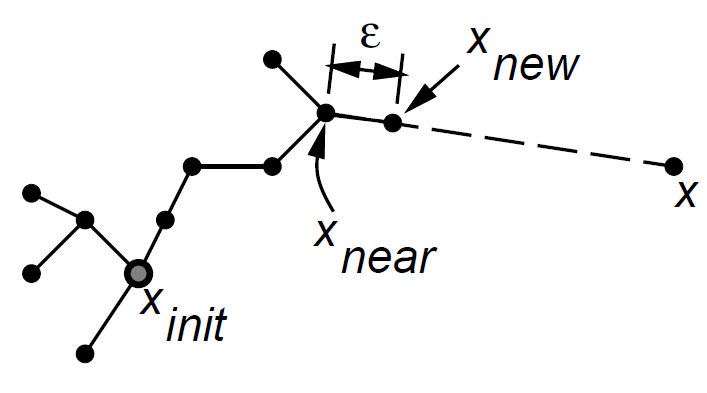
\includegraphics[scale=0.5]{Bilder/Extend.png} 
\caption{Die EXTEND Funktion \citep{Lav00} }
\label{fig3}
\end{figure} \\
Nun wird mit \verb|Collisionfree(x_new, x_near, u)| überprüft, ob \verb|x_new| oder die Bewegung $u$ zu \verb|x_new| hin mit Hindernissen kollidiert oder diesen zu Nahe kommt. Falls dies nicht der Fall ist, werden sowohl der neu entstandene Knoten \verb|x_new| als auch die Kante von \verb|x_near| zu \verb|x_new| dem Baum $T$ hinzugefügt. \\
Falls  \verb|x_new| oder die Bewegung u zu  \verb|x_new| mit Hindernissen kollidiert oder diesen zu nahe kommt, wird der Knoten  \verb|x_new| verworfen und die Funktion \verb|EXTEND(T,x)| beendet.\\

\subsubsection{Vor- und Nachteile von RRT}
Die Rapidly-Exploring Random Trees haben einige Eigenschaften, die für die Bewegungsplanung von Robotern von großem Vorteil sind, wie LaValle in  \citep[Kapitel 3 in][]{Lav98} schreibt:
\begin{enumerate}
\item Ein \textit{RRT} breitet sich sehr schnell in unerforschte Bereiche des Statusraums aus. Dadurch können Pfade schnell gefunden werden und es wird schnell eine mögliche (wenn auch nicht optimale) Lösung gefunden.
\item Die Verteilung der Knoten im Baum entspricht der Verteilung, wie diese Knoten erzeugt wurden; dies führt zu konsistentem Verhalten. Unter anderem kann dadurch das Wachstum des Baumes in eine bestimmte Richtung gesteuert werden (z.B. zum Ziel hin).
\item Ein \textit{RRT} ist probabilistisch vollständig, das heißt mit zunehmender Laufzeit konvergiert die Wahrscheinlichkeit, keinen Pfad zum Ziel zu finden, gegen null.
\item Ein \textit{RRT} ist sowohl einfach zu implementieren als auch einfach in der Analyse, was es ermöglicht, die Geschwindigkeit zu untersuchen und zu verbessern.
\item Ein \textit{RRT} ist immer mit sich selbst verbunden und das bei einer minimalen Kantenanzahl.
\item Ein \textit{RRT} kann als Pfadplanungsmodul interpretiert werden, was die Kombination mit anderen Werkzeugen zur Bewegungsplanung möglich macht.
\end{enumerate}
Leider existieren neben den oben genannten Vorteilen auch etliche Nachteile. Eines der größten ist, dass ein \textit{RRT} nicht den optimalen Pfad zurückliefert, da einmal gesetzte Knoten ihren Vaterknoten nicht mehr ändern können. Dadurch kann, auch wenn durch Neuverknüpfung eine bessere Knotenfolge vom Start zum Ziel bestehen würde, diese nicht erstellt werden. Außerdem bereichern Knoten, die innerhalb des bereits bestehenden Baumes hinzugefügt werden, selten den RRT.\\

\begin{figure}[htb]
    \centering
   \label{fig:fig7}   
 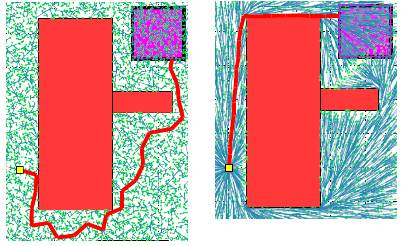
\includegraphics[scale=1]{Bilder/RRT_RRT_star.png} 
 \caption{RRT(links) und RRT* (rechts) mit jeweils 20.000 Knoten}
      
\end{figure}

Deshalb wurde von Sertac Karaman und Emilio Frazzoli aufbauend auf \textit{RRTs} der Algorithmus\textit{ RRT*} eingeführt, welcher diesen Nachteil ausgleicht(siehe Abbildung 2).
\subsection{RRT*}
\label{RRT*}
Im Gegensatz zu einem \textit{RRT} führt ein \textit{RRT*} die zwei folgenden Neuerungen ein:
\begin{enumerate}
\item Auswahl eines passenden Vaterknotens bei Hinzufügen des Knotens zum Baum
\item Neuverknüpfung des Baumes
\end{enumerate}
Diese Neuerungen resultieren in einer veränderten \verb|EXTEND(T,x)| Funktion, siehe \citep{KaFra10}.
\subsubsection{Funktionsweise RRT*}
\begin{lstlisting}
EXTEND(T,x)
	x_nearest = NEAREST_NEIGHBORS(x, T, M);
	x_new = project(x, x_nearest, u);
	if (Collisionfree(x_new, x_near, u) then
		T.add_vertex(x_new);
		x_min= x_nearest;
		c_min = x_nearest.cost + cost(x_nearest, x_new);
		X_NEAR = NEAR_NEIGHBORS(x, T, r);
		foreach x_near in X_NEAR do
			if Collisionfree(x_near, x_new) && x_near.cost + cost(x_near, x_new) < c_min then
				x_min = x_near;
				c_min = x_near.cost + cost(x_near, x_new);
		T.add_egde(x_min, x_new);
		foreach x_near in X_NEAR do
			if Collsionfree(x_new, x_near) && x_new.cost + cost(x_new, x_near) < x_near.cost then
				T.del_edge(x_near_parent, x_near);
				T.add_edge(x_new, x_near);
		Return Extended;
	else
		Return Trapped;
\end{lstlisting}

Während, wie beim Erstellen eines \textit{RRT}, auch bei \textit{RRT*} zuerst der nächste Nachbar als Vaterknoten festgelegt wird, folgt daraufhin ein Speichern der nächsten Nachbarn von \verb|x_new| in einem gewissen Radius $r$ in der Liste \verb|X_NEAR|. 
Es wird \verb|x_min| als der Abstand zum nächsten Knoten gesetzt. Die Funktion \verb|x_nearest.cost| liefert die Kosten, um vom Startknoten zu \verb|x_nearest| zu kommen, zurück, während die Funktion \verb|cost(x_nearest, x_new)| die Kosten des Pfades von \verb|x_nearest| zu \verb|x_new| berechnet. Als vorläufiger Startwert beinhaltet \verb|c_min| demnach die Kosten, um vom Startknoten aus zu \verb|x_new| zu kommen. \\
Die Liste \verb|X_NEAR| wird auf den besten Vaterknoten, also den mit den geringsten Kosten für \verb|x_new|, überprüft. Dieser beste gefundene Nachbar wird für \verb|x_new| als Vaterknoten gesetzt, also eine Kante zwischen \verb|x_new| und \verb|x_near| gezogen. \\
\label{sec:rewiring}
Nachdem so ein Pfad vom Vaterknoten zu \verb|x_new| gebildet wurde, wird der Baum neu verknüpft. Bei jedem Knoten innerhalb des Radius von \verb|x_new| wird überprüft, ob die Kosten mit \verb|x_new| als Vaterknoten geringer werden. Wo immer dies der Fall ist, wird \verb|x_new| als Vaterknoten gesetzt.
\subsubsection{Vor- und Nachteile der Rapidly-Exploring Random Trees*}
\label{sec:rrt*}
Eine Verbesserung zu einem \textit{RRT} ist, dass nicht der nächste Nachbar als Vaterknoten gesetzt wird, sondern der mit den besten Kosten. Je nach Wahl des Radius $r$ und Güte der Kostenfunktion kann hier einiges an \glqq Umweg\grqq{} gespart werden. \\
Der Hauptunterschied ist jedoch die Neuverknüpfung bereits bestehender Knoten über \verb|x_new|. Ein Nachteil des \textit{RRTs} ist, dass Knoten, die aus bereits gut mit Knoten gefüllten Regionen neu hinzugefügt wurden, wenig neues beitragen, also weder neue Regionen entdecken, noch bestehende Pfade verbessern. Dies ändert sich nun, denn jeder von Knoten umgebene, neu hinzugefügte Knoten verbessert die Kosten aller Knoten, die durch \verb|x_new| besser erreichbar sind. Das führt dann sogar soweit, dass ein \textit{RRT*} asymptotisch optimal ist, d.h. bei genügend langer Laufzeit der Pfad zum Optimum konvergiert. Jeder Knoten hilft entweder, den Baum zu expandieren oder sorgt für bessere Pfade innerhalb des Baumes (\citep[vgl. Kapitel 5 in][]{KaFra10}). Je nach Art der Kostenfunktion und dem Samplen neuer Knoten kann der RRT* auch mit bestimmten Eigenschaften ausgestattet werden, z.B. präferiertes Wachsen in bestimmte Richtungen.

Als nächstes werden die Hardware und das verwendete Framework ROS - Robot Operating Systems - vorgestellt. \\
Anschließend werden potentielle Metriken und Datenstrukturen präsentiert.
Bevor wir uns dann den notwendigen Anpassungen des \textit{RRT*}-Algorithmus widmen können, werden die kinematischen und physikalischen Beschränkungen des Autos analysiert.
\subsection{Hardwareausstattung der Autos}
Das Dahlem Center for Machine Learning and Robotics arbeitet mittlerweile mit dem Modellfahrzeug AutoNOMOS Mini v3 (1:10).
\begin{figure}
\centering
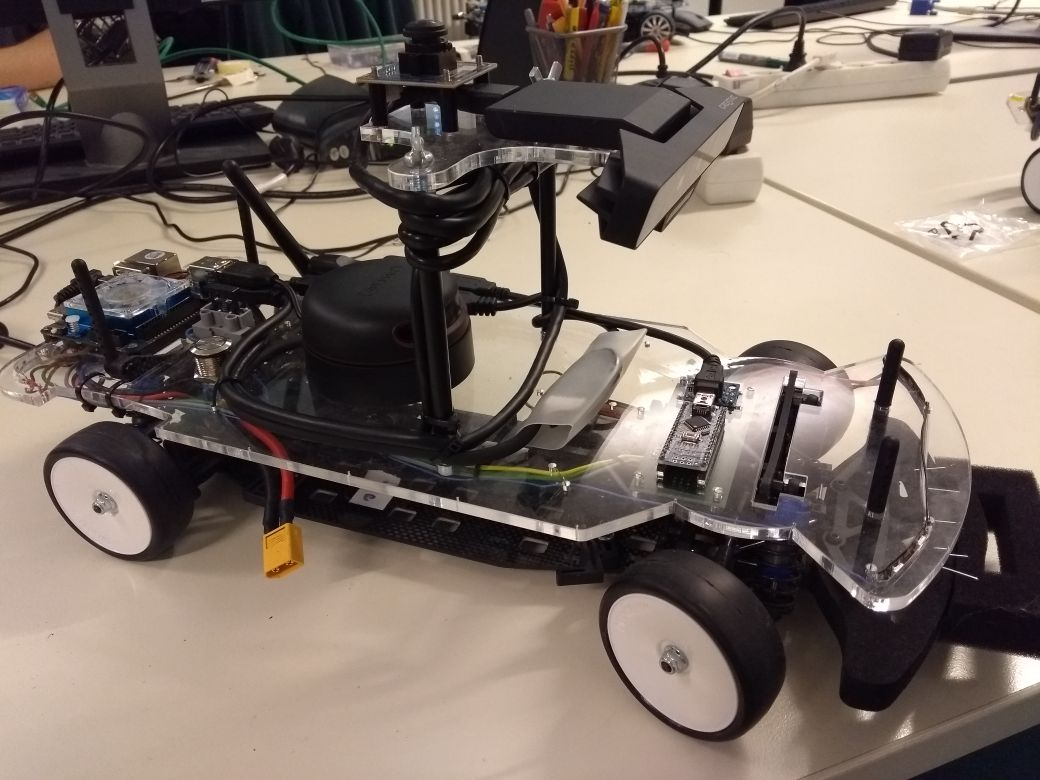
\includegraphics[scale=0.3]{Bilder/car.jpg} 
\caption{Autonoms Mini v3 (1:10)}
\end{figure}
 Der Hauptcomputer des Autos ist ein \textit{Odroid}(XU4 64GB) mit Ubuntu Linux als Betriebssystem und ROS (Robot Operation Systems) zur Steuerung \citep{fubAuto}.\\
\begin{figure}
\centering
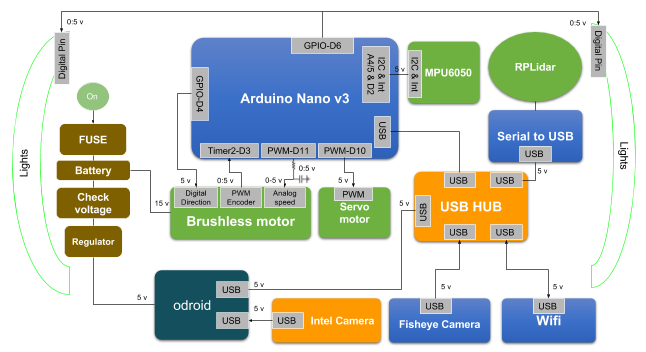
\includegraphics[scale=0.8]{Bilder/AutoNOMOS_mini_v3.png} 
\caption{Überblick über die Module des AutoNOMOS Mini v3}
\end{figure}
Motorisiert ist das Auto mit einem bürstenlosen DC-Servomotor FAULHABER 2232. Die Lenkung wird von dem Servomotor HS-645-MG übernommen; beide Motoren werden mithilfe einer \textit{Arduino Nano} Platine gesteuert. \\
Zur Wahrnehmung der Umgebung besitzt das AutoNOMOS Mini v3 mit dem RPLIDAR A2 360 einen rotierenden Laserscanner, der in der Lage ist, die Umgebung des Autos auf Hindernisse zu überprüfen. Als Rückgabewert liefert der RPLIDAR pro Gradwinkel einen Wert in Metern, wie weit das nächste Hindernis in dieser Richtung entfernt ist, insgesamt also 360 Werte. \\
Auf dem oberen Teil des Autos befestigt ist das \textit{Kinect-type stereoscopic system} (Intel RealSense SR300), welches eine Wolke aus 3D Punkten liefert, die dazu benutzt werden kann, Hindernisse zu erkennen. Außerdem kann die Kamera des \textit{Kinect-type} Sensors dazu benutzt werden, Fahrbahnmarkierungen und Objekte direkt vor dem Auto zu lokalisieren.\\
Der letzte äußere Sensor, auch am oberen Teil des Autos angebracht, ist die Fischaugen-Kamera. Diese zeigt nach oben zur Decke, und kann dazu benutzt werden bestimmte markante, feststehende Objekte zu lokalisieren, damit das AutoNOMOS Mini v3 sich auch innerhalb von Räumen orientieren kann. Dazu kann eine GPS Navigationseinheit simuliert werden, indem die an der Decke angebrachten vier Lampen in unterschiedlichen Farben leuchten.
Die Sensoren sind entweder via USB 3.0 an der Hauptplatine oder direkt am \textit{Odroid} angeschlossen. \\
An inneren Sensoren besitzt das AutoNOMOS Mini v3 eine MPU6050, die einen Beschleunigungssensor und ein \textit{Gyroskop} enthält. Mithilfe dieser MPU kann das AutoNOMOS Mini v3 seine Orientierung, seine Richtung im Raum bestimmen. Außerdem können Messungen zur \textit{Odometrie} ergänzt werden.\\
Das AutoNOMOS Mini v3 wird über eine 14,8 V Batterie mit Energie versorgt.

\subsection{Software: ROS - Robot Operating Systems}
ROS stellt Bibliotheken und Werkzeuge zur Verfügung, die Software-Entwicklern helfen sollen, Robotik-Anwendungen zu kreieren \citep{ROS}. Unter anderem beinhaltet ROS Gerätetreiber, Bibliotheken, Visualisierungswerkzeuge, Paketmanagement und vieles mehr. ROS ist quelloffen und unter der BSD Lizenz verfügbar.
\subsubsection{Architektur}
Mithilfe von ROS können ausführbare Programme, auch Knoten genannt, erzeugt werden, die über so genannte \textit{Topics} kommunizieren können. Dies passiert über einen anonymisierten Publisher/Subscriber Mechanismus, das heißt Daten generierende Knoten können auf relevanten \textit{Topics} Nachrichten senden und Knoten, die Daten benötigen, können von relevanten \textit{Topics} Nachrichten empfangen. \\
Für jedes \textit{Topic} ist dabei auch die Nachrichtenart definiert, die für dieses \textit{Topic} veröffentlicht und von diesem \textit{Topic} empfangen werden. Diese kann neben simplen Datentypen auch aus komplexen, selbst definierten Datenstrukturen bestehen. Dabei wird nur dieser eine, vorher festgelegte Datentyp der Nachricht vom \textit{Topic} akzeptiert.
\textit{Topics} stellen nur eine unidirektionale Verbindung zur Verfügung. Für die Abwicklung von zum Beispiel Remote Procedure Calls sind sogenannte Services zuständig. Diese ermöglichen eine Antwort auf eine bestimmte Anfrage nach dem Client Server Prinzip zurückzusenden.
\subsection{APIs und Einbettung zu bereits vorhandene Knoten}
Das Dahlem Center for Machine Learning and Robotics entwickelte ROS-Pakete für die Steuerung ihrer autonomer Fahrzeuge. Diese Pakete und daraus resultierenden ROS-Nodes können dazu genutzt werden, den von mir entwickelten RRT*-Pfadplaner möglichst gut einzubetten. So kann durch das visuelle indoor GPS die Position des Autos bestimmt werden, die der Pfadplaner für seine Berechnungen braucht. Die resultierende \textit{Trajektorie}, die der Pfadplaner entwickelt, wird dem Low-Level-Planer übergeben, der diese \textit{Trajektorie} in Motorbefehle, also Beschleunigungen und Lenkungen, umsetzt. 
\subsubsection{Bestimmung der Odometrie und visuelles GPS}
Zur Ausführung des Algorithmus gehört, dass das Auto sich selbst lokalisieren kann und seine eigene Startposition feststellen kann. Diese wird mit der aktuellen Ausrichtung des Autos dazu benutzt, den Startpunkt für den Algorithmus zu setzen. \\
Das Dahlem Center for Machine Learning and Robotics hat dafür zwei verschiedene Varianten entwickelt, die sich kombiniert gegenseitig ergänzen können. \\
\begin{enumerate}
\item Odometrie \\
Anhand des Lenkwinkels und der Motordrehgeschwindigkeit kann die erwartete Position, Geschwindigkeit und Beschleunigung berechnet werden. Mit dem im Auto verbauten Gyroskop werden Lageänderungen entlang jeder Achse gemessen. Aufgrund mechanischer Beschränkungen und Ungenauigkeiten sind Messungen mithilfe der Odometrie nie ganz exakt und somit kann eine so bestimmte Position mit der Zeit von der tatsächlichen Position abweichen.
\item Visuelles GPS\\
Da es innerhalb von Gebäuden Schwierigkeiten mit der genauen Positionsbestimmung via GPS gibt, wurde mithilfe von vier Lampen, die an der Decke angebracht wurden, ein visuelles GPS simuliert. Diese vier Lampen leuchten in unterschiedlichen, gut erkennbaren Farben und werden mit der Fischaugenkamera, die zur Decke ausgerichtet ist, erfasst. Anhand der Lage der Lampen zueinander und wie die Fischaugenkamera diese sieht, kann die Position des Autos bestimmt werden.\\
Dazu muss jedoch gesagt werden, dass das eindeutige Erkennen der Lampen nur unter guten Bedingungen (Lichtverhältnisse, alle 4 Lampen im Bild) möglich ist. 
\end{enumerate}

\subsubsection{Low-Level-Planer}
Das Dahlem Center for Machine Learning and Robotics entwickelte den Low-Level-Planer "fub controller", der für die Steuerung der Motoren zuständig ist.
Dieser Planer lauscht auf das \textit{Topic} \verb|"planned_path"|. Auf \verb|"planned_path"| kann eine \textit{Trajektorie} publiziert werden, die dann mithilfe des Low-Level-Planers vom Auto abgefahren wird. Dabei kümmert sich dieser Planer allerdings nicht um etwagige Hindernisse, die mit dem Auto kollidieren könnten, sondern fährt nur die Trajektorie ab. Somit muss der Pfadplaner selbst alle Kollisionen mit Hindernissen ausschließen. \\
Das Format der \textit{Trajektorie} wurde von der Arbeitsgruppe der FU Berlin definiert und besteht aus
\begin{itemize}
\item \verb|std_msgs/Header|: Hier wird die aktuelle Zeit gespeichert.
\item \verb|string child_frame_id|: [TODO] frame id for Twists (velocity and acceleration)
\item \verb|fub_trajectory_msgs/TrajectoryPoint[] trajectory|: Eine Liste aus Trajektorie-Punkten.
\end{itemize}
Ein Trajektorien-Punkt symbolisiert einen abzufahrenden Knotenpunkt und besteht wiederum aus
\begin{itemize}
\item \verb|geometry_msgs/Pose pose|: Hier sind Position und Orientierung des Autos gespeichert.
\item \verb|geometry_msgs/Twist velocity|: Hier wird die Geschwindigkeit des Autos an diesem Punkt gespeichert.
\item \verb|geometry_msgs/Twist acceleration|: Hier wird die Beschleunigung des Autos an diesem Punkt gespeichert.
\end{itemize}
Die Position wird in x-Position und y-Position ausgehend von einer Ecke des Raumes angegeben. Die Orientierung wird durch ein \textit{Quaternion} dargestellt, bei dem durch vier Werte die Drehung in jeder Richtung des Raumes genau bestimmt ist. Allerdings genügt uns die Drehung um die z-Achse, also die Drehrichtung über die Vertikalachse, weshalb dieses Quaternion in einen Winkel, der sogenannten Gierung( engl. \textit{yaw}), umgerechnet wird.
\\

\subsection{Datenstruktur}
Um die Anwendung in Echtzeit zu nutzen, muss die Geschwindigkeit des RRT* Algorithmus sehr hoch sein. Der gesamte Algorithmus, bestehend aus Aufbau des Baumes, Rewiring, dem Finden einer gültigen Trajektorie vom Start zum Ziel und Vermeiden von Hindernissen sollte nicht mehr als 250 Milisekunden brauchen. Dadurch wird gewährleistet, dass auch sich bewegende Hindernisse stets erkannt werden und der Pfad des Autos gültig bleibt. \\
RRT* erzeugt n Punkte. Jeder dieser Punkte sucht zuerst seinen nächsten Nachbarn, dann wird der Punkt an den Baum projiziert und dem Baum hinzugefügt. Am Ende wird der Baum neu verknüpft. \\
Unter der Voraussetzung, dass die Suche des nächsten Nachbarn in der Zeit O(log n) zu bewerkstelligen ist, hat RRT* eine Laufzeit von O(n log n). Dies ist jedoch nur durch die Wahl einer passenden Datenstruktur zu erreichen, die \textit{k-nearest neighbour} Suche und \textit{radius k-nearest neighbour} in O(log n) durchführen können.\\
Es existieren bereits viele wissenschaftliche Untersuchungen und auch empfohlene Datenstrukturen, wie zum Beispiel k-d-Bäume \citep{Bentley75}. Leider benötigt der RRT* Algorithmus eine dynamische Datenstruktur, da Punkte erst nach und nach hinzugefügt werden. Das Hinzufügen eines Punktes muss somit auch in logarithmischer Zeit gewährleistet sein. \\

Aufgrund fehlender Implementierungen und Mangel an Zeit zum Erstellungszeitraum dieser Arbeit konnte eine solche Datenstruktur nicht mehr im Zusammenhang mit dieser Arbeit implementiert werden. Der alternative Versuch, mit nanoflann \citep{blanco2014nanoflann}, die Knoten in einen KD-Baum zu verwenden, scheiterte an der fehlenden dynamischen Unterstützung.\\

Deshalb wurde versucht, eine einfachere Datenstruktur mit den ersehnten Eigenschaften zu entwerfen. Dazu wurde ein einfaches Gitter implementiert, deren Achsen die x- und y-Werte des einzufügenden Punktes repräsentierten. Dadurch fallen Punkte, die nah beeinander sind, in die gleiche oder benachbarte Zellen. Je nach Wahl der Größe der Zellen müssen nur die Knoten der Zelle selbst und der Nachbarzellen überprüft werden. Ein weiterer Vorteil des Gitters ist das schnelle Einfügen eines Knotens: Dadurch dass das Gitter statisch bleibt, können Arrays als Rahmen gewählt werden und die Laufzeit zum Einfügen von Knoten liegt bei O(1).\\
Im optimalen Fall muss bei der \textit{k-nearest neighbour} Suche nur die Zelle, worin der Knoten liegt, sowie alle acht angrenzenden Zellen untersucht werden. Solange sich allerdings nur sehr wenige Knoten im Gitter befinden, muss unter Umständen das gesamte Gitter nach Nachbarn abgesucht werden, was die Laufzeit stark verschlechtert. Innerhalb einer Zelle sind die Knoten in einer Liste gespeichert. Sollten sehr viele Knoten in eine Zelle fallen, dauert das Durchsuchen dieser Zelle sehr lange. Wird also die Zellgröße groß gewählt, dauert das Durchsuchen einer Zelle lange, wird sie klein gewählt, müssen zu viele Zellen durchsucht werden. \\
Aufgrund einer zu hohen Laufzeit und Fehleranfälligkeit wurde das Gitter verworfen und zur Speicherung der Knoten eine einfache Liste gewählt. Dadurch hat der Algorithmus zwar eine Laufzeit von O($n^2$), dafür waren die Fehleranfälligkeit und der zeitliche Implementierungsaufwand nicht so hoch. \\
\subsection{Sonstige verwendete Software}
Anfangs wurde in der Programmiersprache Python programmiert. Zur Verbesserung der Geschwindigkeit wurde jedoch schnell zu C++ gewechselt. Als Entwicklungsumgebung wurde Eclipse mit dem CTD-Plugin gewählt. \\
Zur Berechnung der Vektorarithmetik wurde die C++ Headerbibliothek Eigen3 verwendet.

Nachdem die notwendige Infrastruktur und verwendete Software erläutert wurde, folgt eine kurze Betrachtung der kinematischen und physikalischen Einschränkungen, denen das AutoNOMOS Mini v3 unterworfen ist. Anschließend wird sich im Folgenden dem Kernstück der Arbeit, dem eigentlichen RRT*-Pfadplaner, gewidmet.
\subsection{Kinematische und physikalische Einschränkungen}
Im Gegensatz zu holonomischen Fahrzeugen, die sich ohne Einschränkungen in alle Richtungen des Raumes bewegen können, sind die möglichen Pfade eines nicht holonomischen Fahrzeug wie ein Auto nicht so einfach zu berechnen. Deshalb stellen wir zuerst ein mathematisches Modell des Autos auf und definieren die Randbedingungen, unter denen es agiert.
Die mathematischen Definitionen der Randbedingungen und des Autos sind in der Bachelorarbeit von David Gödicke \citep{Goedicke18} gut beschrieben und werden hier übersetzt übernommen. \\
\subsubsection{Randbedingungen}
Die Position des Autos bezieht sich auf den Mittelpunkt zwischen den Hinterrädern mit den Koordinaten x und y. Der Winkel $\theta \in S,  S=[0,2\pi]$ steht für die Ausrichtung des Autos, der Winkel $\phi \in S$ für die Ausrichtung der Räder (=Lenkwinkel). Wir nehmen an, dass das Auto sich auf einer flachen Ebene bewegt. Somit ist der Arbeitsraum definiert durch $C =  \mathbb{R \times S}$. Ein Zustand des Autos wird beschrieben durch $q \in C = (x,y,\theta)$.\\
Zur Vereinfachung der Rechnungen wird angenommen, dass die Räder bei Bedarf sich sofort, ohne Zeitverlust, in die gewünschte Position begeben. Da der Lenkwinkel keinen Einfluss auf den Momentanzustand des Autos hat, wird dieser in der Zustandsbeschreibung nicht aufgeführt. Zusätzlich kommt noch hinzu, dass das Auto zur Testzwecken bestimmte Geschwindigkeiten nicht überschreiten darf, sodass der minimale Kurvenradius nur durch den Lenkwinkel beschränkt ist und nicht auch noch zusätzlich durch die Geschwindigkeit. \\
Die durch den Algorithmus berechnete Trajektorie führt von der Startposition des Autos (Startknoten) über eine Anzahl von Knoten bis zu einem Zielknoten im Zielbereich. Jeder Knoten K ist definiert mit $K= (x,y,\theta, c, V)$. X und y sind die Koordinaten des Knotens, $\theta$ die Ausrichtung, die das Auto in diesem Knoten hätte. C sind die durch eine Kostenfunktion \ref{sec:Kosten} berechneten Kosten, um vom Startzustand zu diesem Knoten zu gelangen und V ist der Vaterknoten. 

\subsubsection{Einschränkungen durch das Auto}
Der Zustand des Autos kann durch Beschleunigung verändert werden. Ein negatives Beschleunigen entsteht beim Bremsen oder Rückwärtsfahren. Zusätzlich zu dieser einen Möglichkeit, den Zustand des Autos zu ändern, kann das Auto das Resultat der Beschleunigung ändern, indem der Lenkwinkel angepasst wird. Dieser reicht von $\phi_{max}$ bis $-\phi_{max}$, den maximalen Lenkwinkeln des Autos.
Je nach Lenkwinkel $i_{\phi}$, Geschwindigkeit $i_g$ und Anfangsausrichtung des Autos $\theta$ ändern sich verschiedene Parameter des Zustandes $q(x,y, \theta) $: \\
\begin{center}
$ \dot{x} = i_g cos \phi $ \\
$ \dot{y} = i_g sin \phi$ \\
$ \dot{{\theta}} = \frac{i_g}{L} tan (i_{\phi}) $
\end{center}
L ist hierbei der Radstand, also der Abstand zwischen der Vorder- und der Hinterachse. \\

